\subsubsection{Versionsverwaltung}\label{vcs}

Ein VCS (auch SCM System genannt) ist eine Software mit der die Änderungen an Dateien nachverfolgt und bei Bedarf wieder zusammengeführt werden können.
Es ermöglicht mehreren Personen Änderungen an dem gleichen Quellcode nachvollziehbar durchführen zu können.
Jeder hat seine eigene Kopie des Quellcodes.
Das zurzeit am meisten verwendete SCM ist Git.
Es wird unter anderem bei Google, Facebook, Microsoft und der Linux Entwicklung verwendet. \footnote{Git Website, vgl.~\cite{GIT_SCM}}
Git ist über die Kommandozeile bedienbar.
Es sind jedoch ebenfalls zahlreiche grafische Tools verfügbar.
Teilweise sind diese auch bereits in Entwicklungsumgebungen (IDE) integriert.

\paragraph{Repository}

Ein Repository ist ein Ordner in dem sich ein \texttt{.git} Ordner befindet.
Hier wird die Historie und alle Branches verwaltet. \footnote{Git Basics, vgl.~\cite{GIT_SCM_BASICS}}
Werden Dateien in diesem auch als \textsl{Working Directory} bezeichneten Ordner verändert, dann lassen sich diese Änderungen mit Git erfassen.
Es wird dabei zwischen \textsl{Unstaged-} und \textsl{Staged}-Änderungen unterschieden.

\paragraph{Remote}

Git ist dezentral.
Ein Repository kann ein oder mehrere Remotes haben.
Dabei handelt es sich um Server auf denen der jeweilige Branch mit einem \textsl{Push} aktualisiert werden kann.
Es muss keine Remotes haben.
So ist es möglich Git auch ohne Internetverbindung zu verwenden.
Der dezentrale Ansatz sorgt dafür, dass jeder Entwickler, auf eine vollständige Kopie des ausgecheckten Codes Zugriff hat.
\footnote{Git Basics - Working with Remotes, vgl.~\cite{GIT_SCM_REMOTES}}

\paragraph{Branch}

Ein Entwicklungszweig, der die versionierten Dateien enthält, wird als \textsl{Branch} bezeichnet.
In der Regel gibt es einen Hauptbranch welcher als \textsl{Master} bezeichnet wird.
Von diesem wird abgezweigt. \footnote{Git Branching - Branches in a Nutshell, vgl.~\cite{GIT_SCM_BRANCHING}}
Jeder Entwickler führt seine Änderungen auf seinem Branch durch und anschließend können diese Änderungen wieder in den Hauptzweig überführt werden.

\paragraph{Commit}

Änderungen die \textsl{Staged} sind können zu einem Commit zusammengefasst werden.
Ein Commit besteht aus den Veränderungen (Diffs) und einer Commit Message vom Entwickler.
Er wird immer auf einem Branch durchgeführt.
Jeder Commit erhält einen Hash-Wert und kann einen Parent-Hash-Wert haben.
Durch diese Hashes kann Git die Änderungshistorie aufbauen und nachvollziehen, wie Änderungen wieder zusammenzuführen sind.

\begin{figure}[htb]
    \centering
    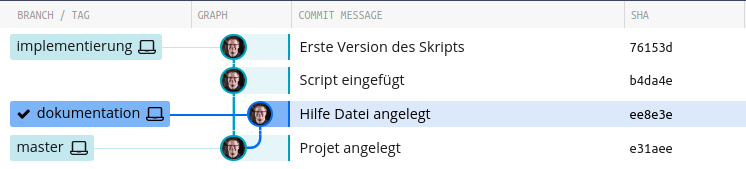
\includegraphics[width=0.8\textwidth]{images/gitkraken_screenshot.png}
    \caption[Commits und Branches in Git]{Commits und Branches in Git}
    \label{fig:Screenshot aus dem Git Client GitKraken}
\end{figure}

\paragraph{Pull/Merge Request}

Um immer einen funktionierenden Stand zu haben wird der Master Branch geschützt, d.h. dass kein direkter Push von Commits auf den Master Branch erfolgen kann.
Damit Code in den Master Branch eingefügt werden kann, werden sogenannte Pull bzw. Merge Request verwendet.
Der Entwickler, der neuen Code auf seinem Branch erstellt hat, erstellt einen Pull Request.
Über die Benutzeroberflächen von Git Kollaborationssoftware (z.B. Gitlab, GitHub, Bitbucket) können so die Änderungen eingesehen und kommentiert werden.
Darüber hinaus kann ein PR/MR dazu verwendet werden auf einem CI Server einen Arbeitsablauf zu starten. \footnote{About pull requests, vgl.~\cite{GITHUB_ABOUT_PR}} \\

%\paragraph{Fork}
%
%- Merge: Führt Änderungen aus einem anderen Branch in den aktuellen Branch ein.
%- Rebase: Hängt die Änderungen auf dem aktuellen Branch an die Änderungen des gewünschten Branches an.
%- Pull/Merge Request:
%- Merge Conflict: Ein Konflikt tritt immer dann auf wenn zwei Entwickler auf unterschiedlichen Branches die gleichen Zeilen bearbeitet haben. Git kann dann nicht mehr unterscheiden welche Änderung genommern werden soll und dieser Konflikt muss manuell aufgelöst werden.
%- Fork: Dieser Begriff kommt vor allem im Zusammenhang mit Open-Source Repositories vor, bei einem Fork erstellt der Entwickler eine Kopie des Repositories in seinem eigenen Account, dort kann er dann Branches anlegen und anschliessend einen Pull Request machen. `(https://docs.github.com/en/free-pro-team@latest/github/getting-started-with-github/fork-a-repo)`

Ein Ansatz aus Scrum und DevOps ist die Annahme, dass der Master Branch immer in einem Zustand ist in dem eine stabile und funktionsfähige Software an den Kunden geliefert werden könnte.
\footnote{Armenise, vgl.~\cite{Armenise2015}~[S.24]}